% Innehållet i Vasungavisor 2010
%
% Kapitel "I Högan Nord"

\songchapter{Auld Acquaintance}
\begin{figure}[!b]
\begin{center}
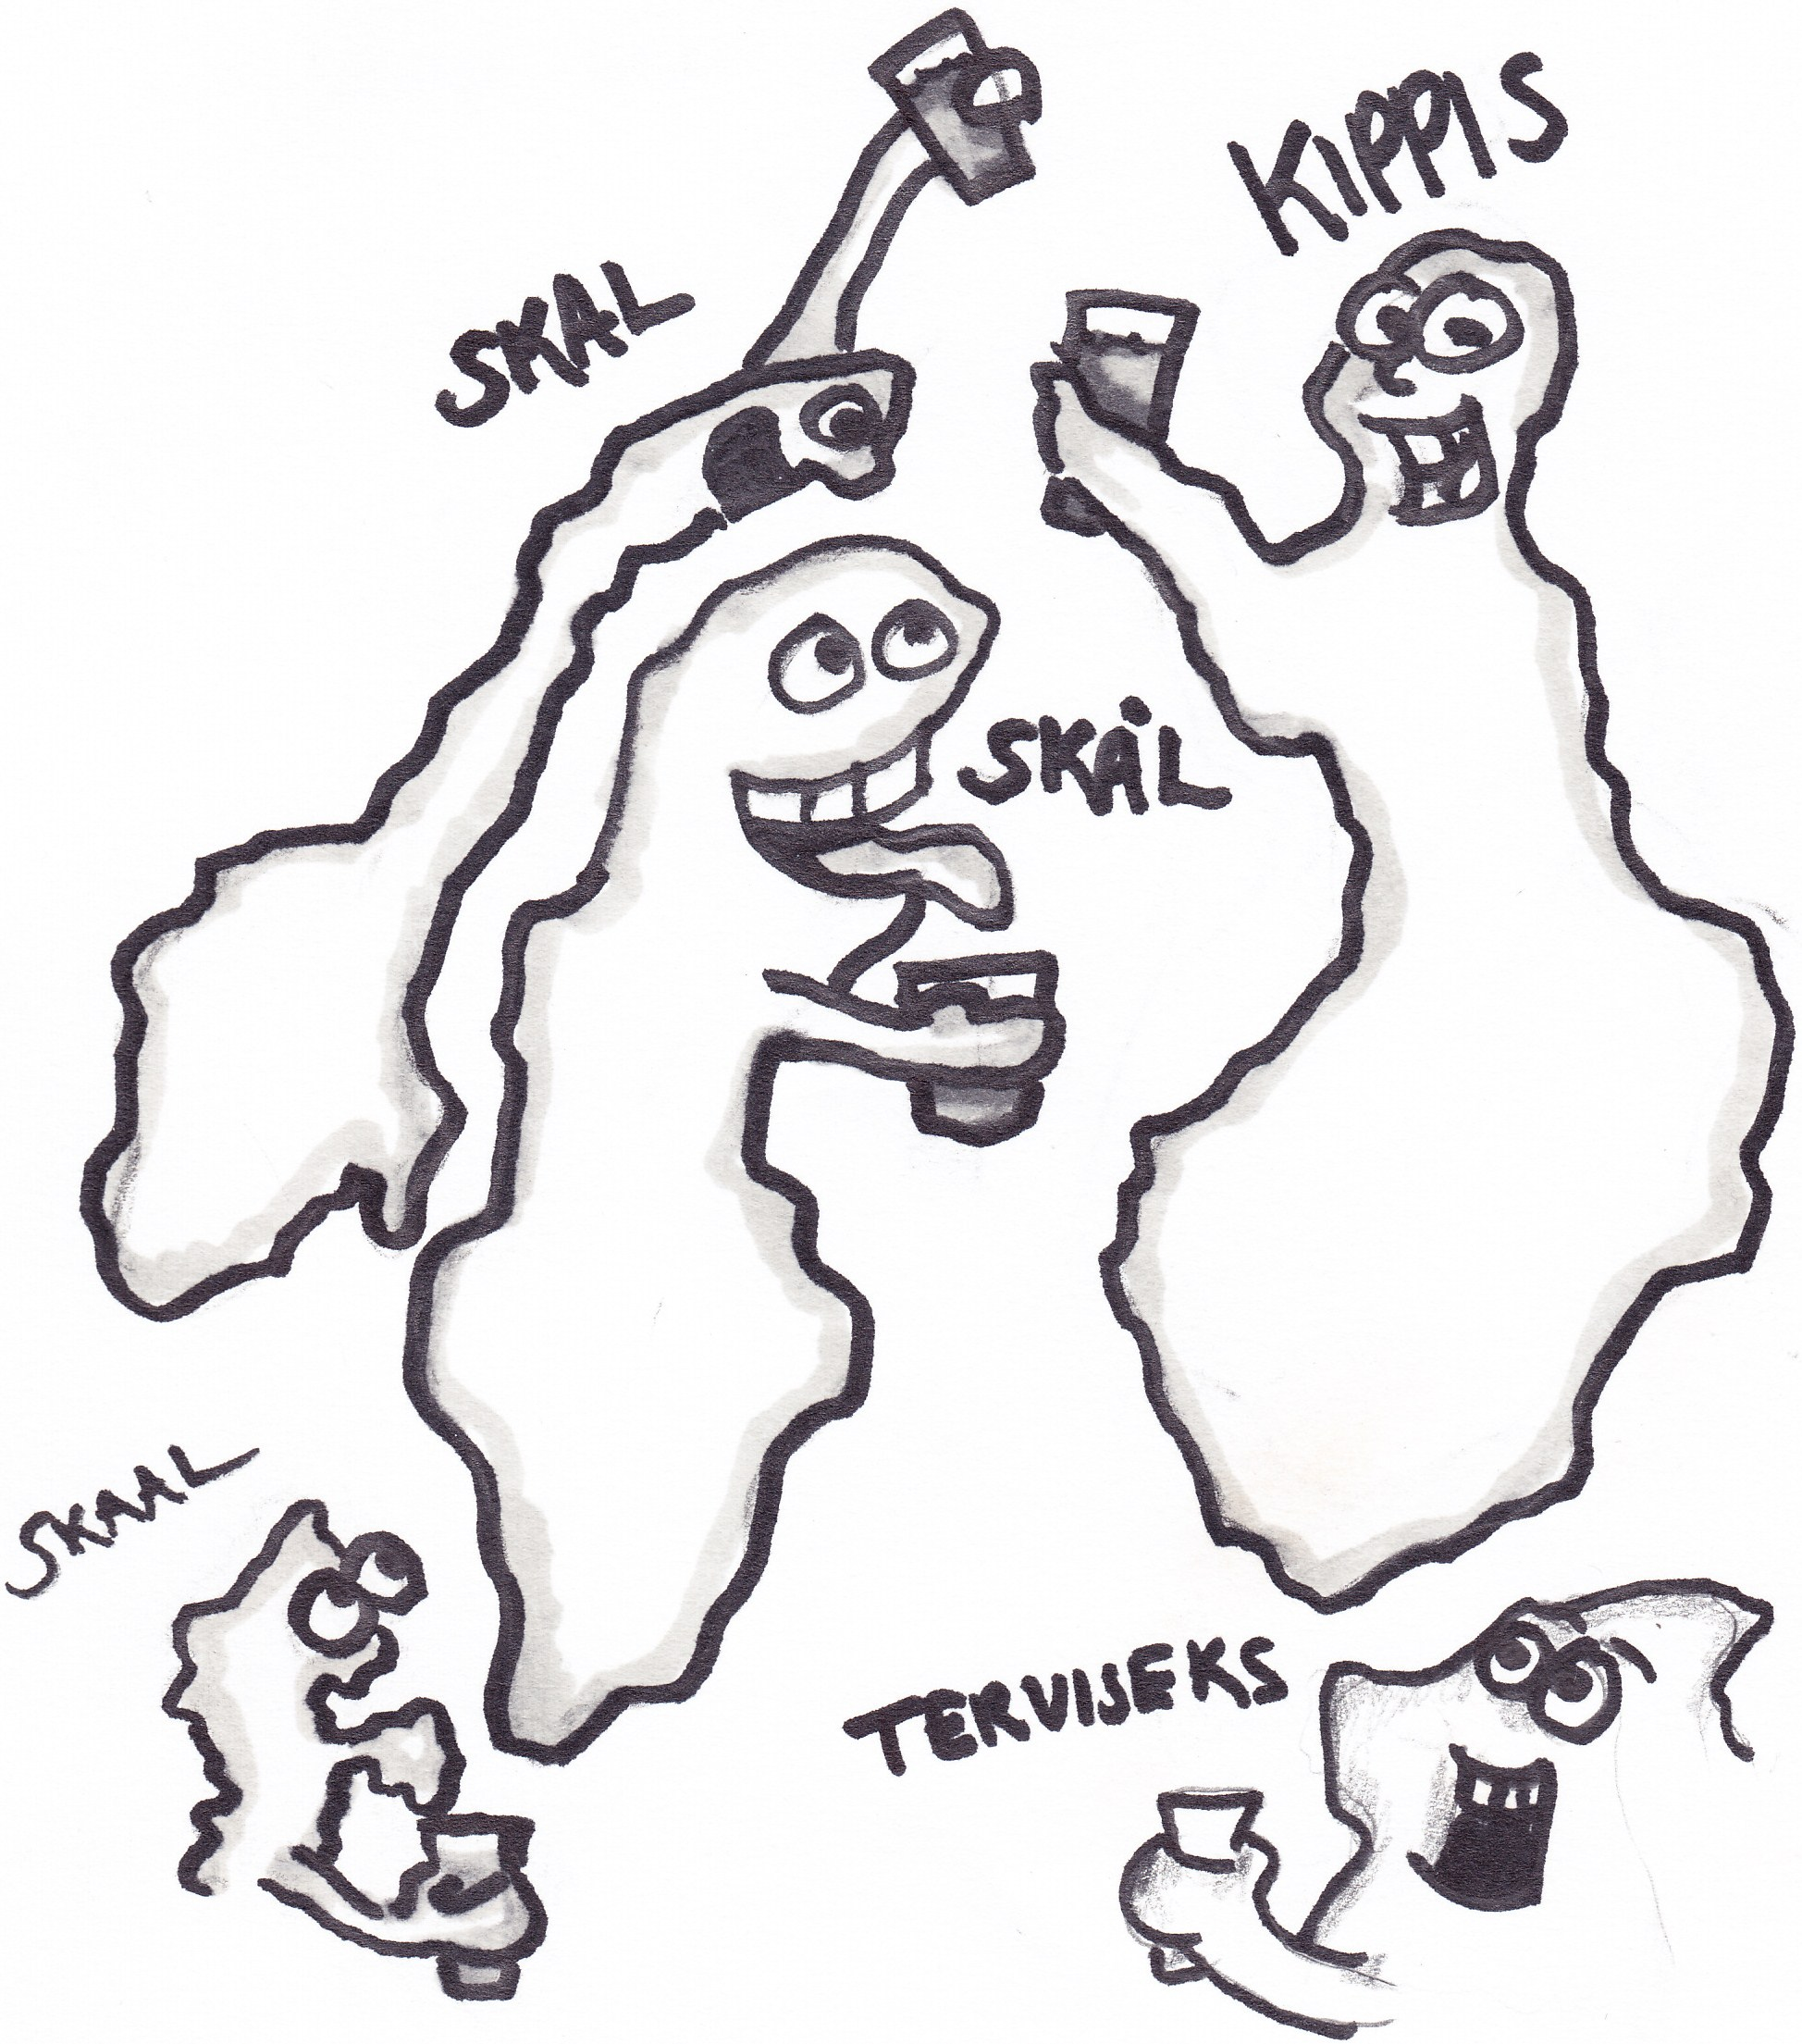
\includegraphics[width=6cm]{../bilder/auld.jpg} 
\end{center}
\end{figure}
\clearpage
\input{JagTrivsBastIOsterbotten.tex}
\clearpage
% Innehållet i Vasungavisor 2010

\beginsong{Norrlandssången Norrlands nation}[
  sr={I Apladalen i Värnamo}]
  
\beginverse*
 Hör du, säg hör du vår norrländska låt
 över vidden klinga, manande och bringa
 hälsning till landet där mångmila ståt
 banande når den bygden som är vår?
 \endverse
 \beginverse*
 Älvarnas silver i mörknande skog.
 Bergsmassiv som gåna och sin märg oss låna.
 Skälvande mylla bak vändande plog.
 Havets vida famn med skötar, grund och hamn.
 \endverse
 Norrland är vårt rike, landet utan like.
 Storvulet vilt eller leende och milt.
 I mitt sinne leka jublande veka
 sånger ibland om min hembygds fagra land.
 \beginverse*
 Lyft då ditt huvud och räta din rygg!
 Stoltare än andra kan du vägen vandra.
 Norrlänning är du och ärlig och trygg.
 Sjung din vandringslåt på norrländsk färdeståt!
\endverse
\endsong




\clearpage
\input{INorrlandVaxerDet.tex}
\begin{figure}[!b]
\begin{center}
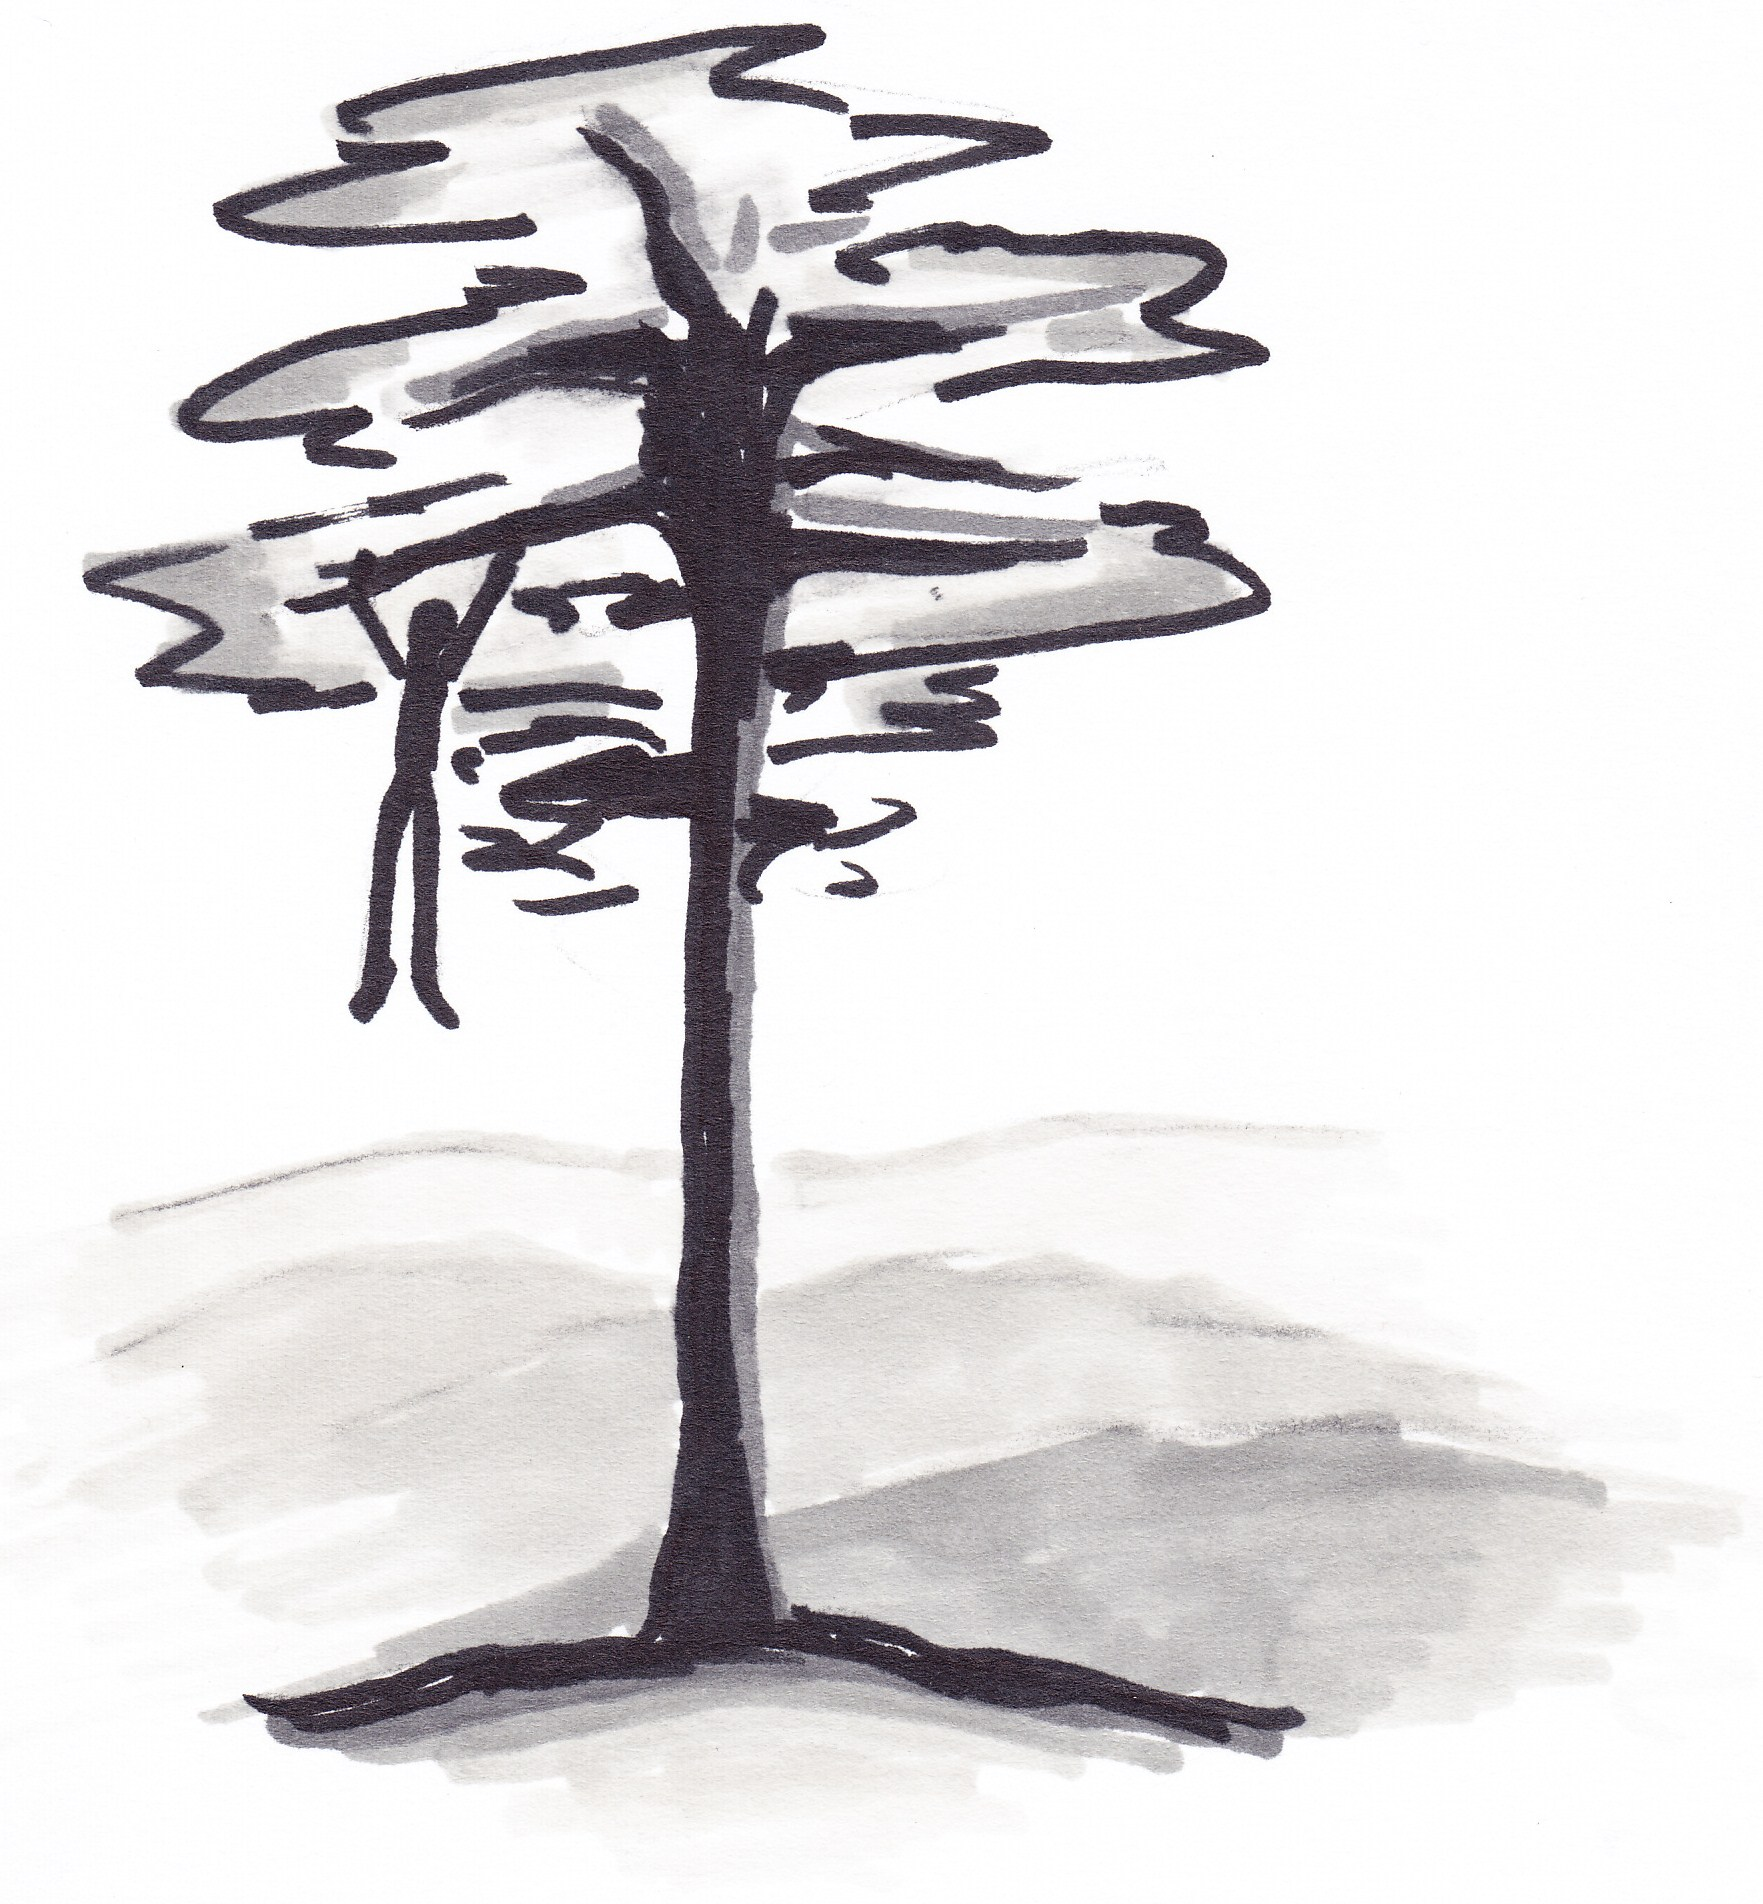
\includegraphics[width=4cm]{../bilder/inorrland.jpg} 
\end{center}
\end{figure}
\clearpage
\input{ViKomFranNorrland.tex}
\clearpage
% Innehållet i Vasungavisor 2010

\beginsong{Grön å vit}[
sr={Mi Lord}]

\beginverse*
/: Jag vill bli grön å vit.
Jag vill bli kalmarit
Oh snälla snälla låt mig bli en kalmarit
Oh ja, poängen dom,
Bryr vi oss inte om,
För i kväll ska vi slå runt här gång på gång…:/
\endverse

\beginchorus
Raj raj raj raj raj raj…
\endchorus
\endsong
\clearpage
\input{Kalmarevisan.tex}
\begin{figure}[!b]
\begin{center}
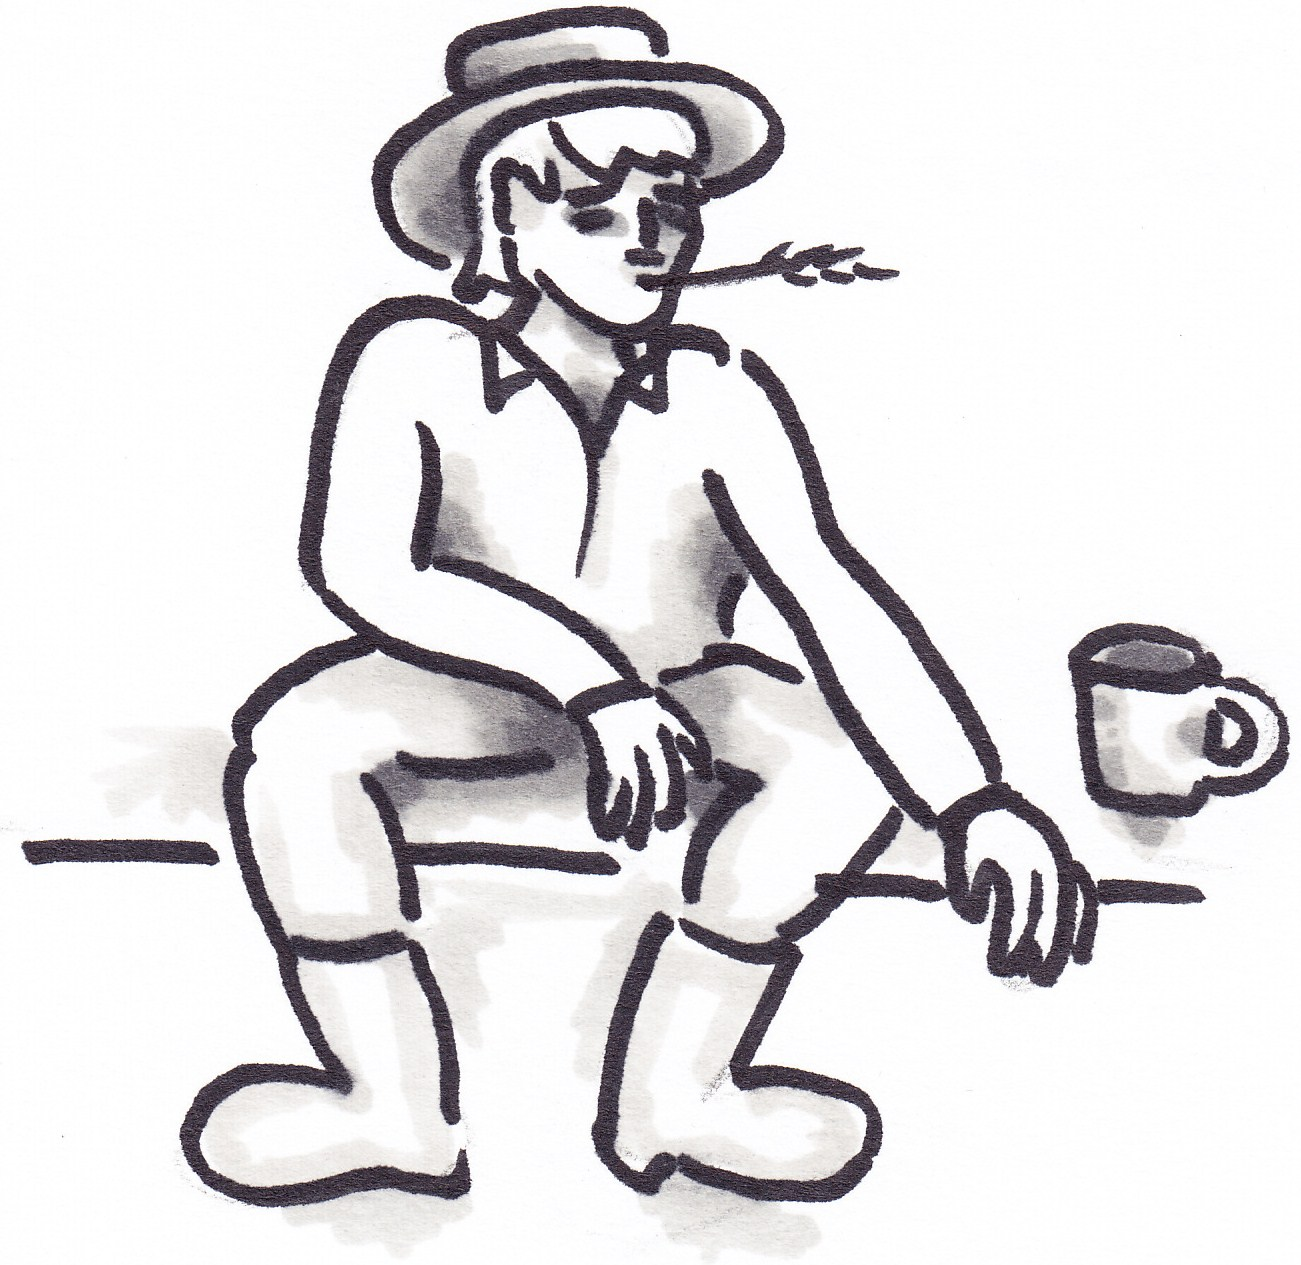
\includegraphics[width=4cm]{../bilder/bonde.jpg} 
\end{center}
\end{figure}
\clearpage
% Innehållet i Vasungavisor 2010

\beginsong{Lossis nimega gradesko}[
	by={Viktor von Scheffel}]
  
\beginverse*
Lossis nimega Gradesko,
kaugemal kui Temesvar,
istus vahva vürst Bibesko, Bibesko!
Serbia hall hospodar. 
\endverse
\beginchorus
:,: Hai-tiri-lal-la, hai-tiri-lal-la, 
hai tiri-lal-la-lal-lal-la. :,: 
\endchorus
\beginverse*
Mida tegi vürst Bibesko,
Serbia hall hospodar,
lossis nimega Gradesko, Gradesko!
kaugemal kui Temesvar?
\endverse
\beginchorus
:,: Hai-tiri-lal-la... :,: 
\endchorus
\beginverse*
Slivovitši jõi Bibesko,
Serbia hall hospodar,
lossis nimega Gradesko, Gradesko!
kuni purjus oli vaar.
\endverse
\beginchorus
:,: Hai-tiri-lal-la... :,: 
\endchorus
\endsong

\clearpage
\beginsong{Me mõtted on priid}[
	by={August Anni}]

\beginverse
Me mõtted on priid,
kes suudaks neid köita?
Kes vägev on nii,
et vangi meid heita?
Ka vanglas ja vaevas
meil lahti on taevas.
:,: Kõikvõimsad me nii —
Me mõtted on priid. :,: 
\endverse

\beginverse
On elada rõõm
kesk päikese kulda,
On harida rõõm
maad emakest mulda.
Ja kannatust kanda
ja ohvriks end anda.
:,: Kõikvõimsad me nii —
Me mõtted on priid. :,: 
\endverse

\beginverse
Kõik muu meil ükskõik,
mis ise m'ei taha.
Meist enestest kõik,
kas hää see või paha.
Me süda ja silmad
need loovad maailma.
:,: Kõikvõimsad me nii —
Me mõtted on priid. :,: 
\endverse
\endsong
\clearpage
\input{Aquaviten.tex}
\begin{figure}[!b]
\begin{center}
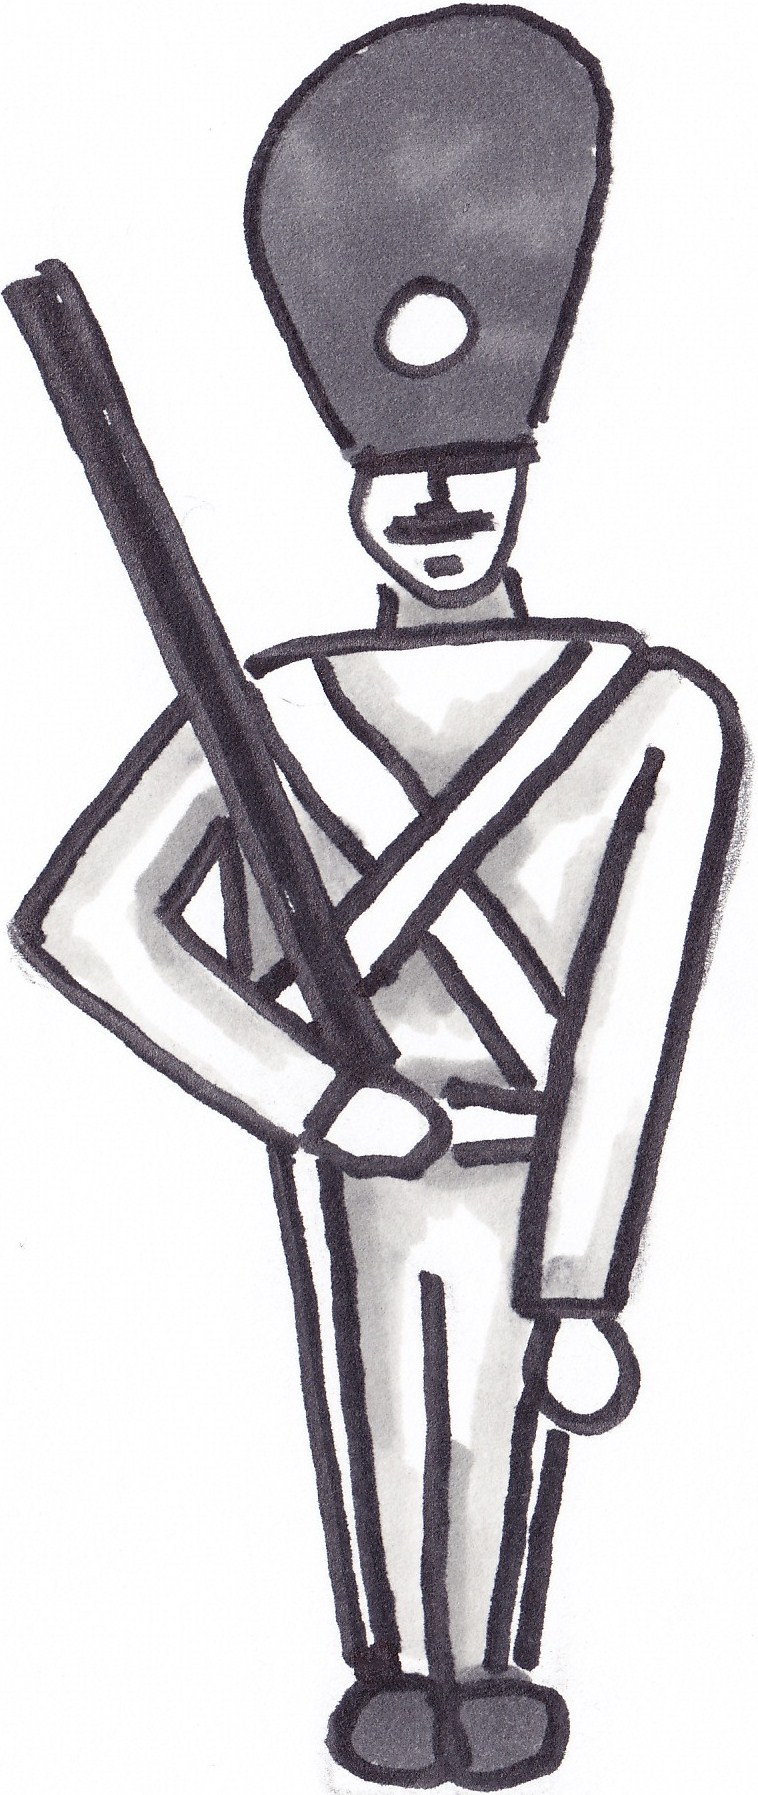
\includegraphics[width=25mm]{../bilder/dansk.jpg} 
\end{center}
\end{figure}
\clearpage
\beginsong{Viina painaa}[
	by={Marjatta Pokela},
		sr={Käki kukkuu kuusikossa}]

\beginverse
Viina painaa, viina painaa,
viina painaa aina.
Kauppakassissa lauantaina
ja päässä sunnuntaina.
\endverse

\beginverse
Viina maistuu, viina maistuu,
viina maistuu aina.
Arkipäivän askareissa
ja vielä sunnuntaina.
\endverse

\beginverse
Vesi loppuu, vesi loppuu,
vaan ei lopu viina.
Veden puute on paha juttu,
mutt' viinan puute on piina!
\endverse
\endsong
\clearpage
% Innehållet i Vasungavisor 2010

\beginsong{Jos eukkosi kieltää}
  
\beginverse*
Jos eukkosi kieltää sua juomasta,
niin juo, niin juo.
Jos kieltää sua viinoja tuomasta,
niin tuo, niin tuo.
Mutt' juomasta älä sinä milloinkaan lakkaa,
vaan hanki sinä itselles' parempi akka.
Ja juo ja laula, ja juo ja laula,
ja juo ja laula, ja juo ja laula...
\endverse

\beginchorus
Trink, trink, Brüderlein trink
lass doch die Sorgen zu Haus
trink, trink, Brüderlein trink
leere dein Glas mit mir aus
Meide den Kummer und meide den Schmertz
dann ist das Leben ein Schertz.
Kauf dir ein Auto und fahr gegen Baum
dann ist das Leben ein Traum
\endchorus

\beginverse*
Upseerit sotia taistelee,
ja juo, ja juo,
ja teltassa viinoja maistelee,
ja juo, ja juo.
Kun taistelun melskeessä pyssyt ne paukkaa,
niin upseerit välillä pullosta naukkaa,
ja juo ja laulaa ...
\endverse

\beginchorus
Trink, trink, Brüderlein trink...
\endchorus

\beginverse*
Maisterit koulussa opettaa,
ja juo, ja juo,
ja illalla tuntinsa lopettaa,
ja juo, ja juo.
Kun päivällä saksaa ja matikkaa jauhaa,
niin illalla raitilla räyhää ja pauhaa,
ja juo ja laulaa ...
\endverse

\beginchorus
Trink, trink, Brüderlein trink...
\endchorus

\endsong

\clearpage
\input{TrinkTrink.tex}
\begin{figure}[!b]
\begin{center}
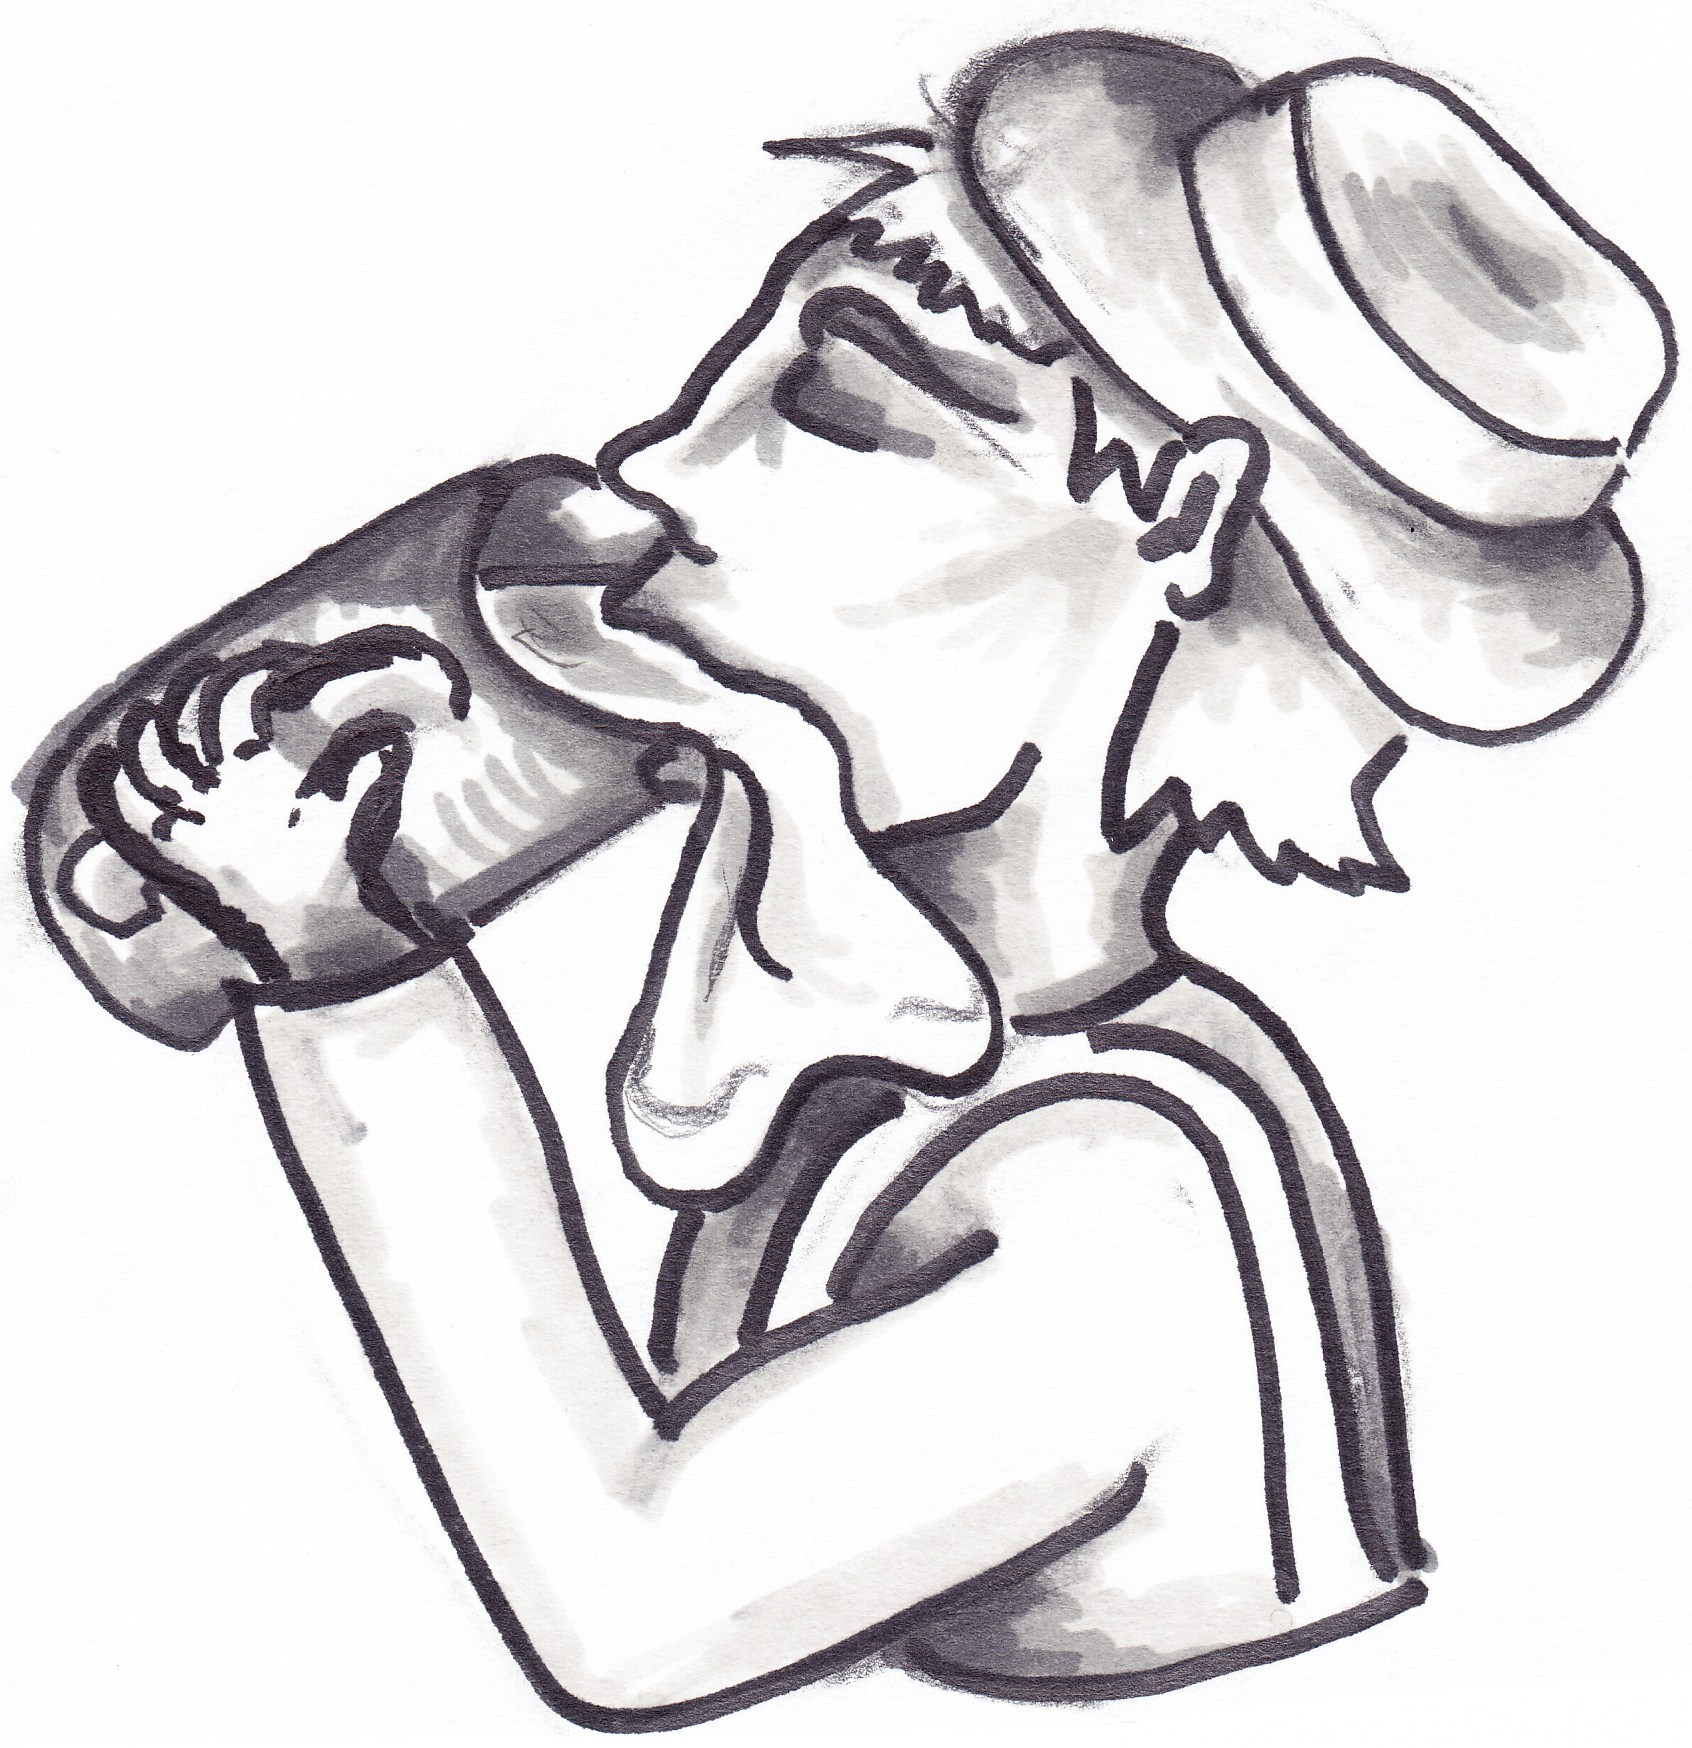
\includegraphics[width=3cm]{../bilder/trinktrink.jpg} 
\end{center}
\end{figure}
\clearpage
\input{Urbummellied.tex}
\clearpage
% Innehållet i Vasungavisor 2010

\beginsong{So troll’n wir uns}[
	by={Carl Zuckmayer},
	sr={Så lunka vi}]
  
\beginverse*                                        
So troll'n wir uns ganz fromm und sacht
von Weingelag und Freudenschmaus,
wenn uns der Tod ruft: Gute Nacht,
Dein Stundenglas rinnt aus.
Wer heut noch frech den Schnabel wetzt
und glaubt, ein großer Herr zu sein,
pass auf, der Schreiner hobelt jetzt
grad schon an deinem Schrein.
\endverse

\beginchorus
Scheint das Grab dir tief und dumpf sein Druck:
Alavott, so nimm noch einen Schluck,
und noch einen hinterher,
und rasch noch zweie, dreie mehr,
dann stirbt sich’s nicht so schwer.
\endchorus

\beginverse*
Der nach des Andren Liebsten schielt
und doch sich fühlt als Nobelmann,
pass auf! Dem Spielmann, der dir spielt,
springst du ins Grab voran!
Und du, der toll vor Eifersucht
zerschmiss einst jedes Glas im Saal –
wenn dich der Tod im Bett besucht –
hoch lebe dein Rival!
\endverse

\beginchorus
Scheint das Grab dir tief...
\endchorus

\beginverse*
Was hilft's, wenn du vor Wut auch spuckst,
der Tod ist keiner Münze feil.
Von jedem Schlückchen, das du schluckst,
schluckt schon der Wurm sein Teil.
Ob niedres Pack, ob hohe Herrn –
am Ende sind wir Brüder doch:
dann leuchtet uns der Abendstern
ins gleiche finstre Loch.
\endverse

\beginchorus
Scheint das Grab dir tief...
\endchorus
\endsong

\clearpage
\input{AuldLangSyne.tex}
\clearpage
% Innehållet i Vasungavisor 2010

\beginsong{What should we do with the drunken sailor?}
  
\beginverse*                                        
What should we do with the drunken sailor 
What should we do with the drunken sailor
What should we do with the drunken sailor 
early in the morning?
\endverse

\beginchorus
Ho-ray and upp she rises,
ho-ray and upp she rises,
Ho-ray and upp she rises,
early in the morning!
\endchorus

\beginverse*
Put him in the long boat until he's sober...
\endverse

\beginchorus
Ho-ray and upp she rises...
\endchorus

\beginverse*
Pull out the plug and wet him all over...
\endverse

\beginchorus
Ho-ray and upp she rises...
\endchorus

\beginverse*
Put him in a bed with the captain's daughter...
\endverse

\beginchorus
Ho-ray and upp she rises...
\endchorus
\endsong

\clearpage
\beginsong{Kuka helvetti}[,
		sr={Polonaise}]

\beginverse
Kuka helvetti heitti kiven mun
viinapulloon? (x 4)
\endverse

\beginverse
Vem i helvete kasta' sten på min
flaska brännvin? (x 4)
\endverse

\beginverse
Who the hell threw this bloody stone at my
whisky bottle? (x 4)
\endverse

\beginverse
Wer zum Teufel warf ein Stein zu mein
Flasche Rheinwein? (x 4)
\endverse

\beginverse
Kes kurat viskas kive minu
viinapudelisse? (x 4)
\endverse

\beginverse
Saku Sammakko heitti kiven mun
viinapulloon! (x 4)
\endverse
\endsong